\documentclass[10pt]{article}
\usepackage[margin=1in]{geometry}
\usepackage{amsmath}
\usepackage{graphicx}
\usepackage{booktabs}
\usepackage{hyperref}
\usepackage{xcolor}
\usepackage[OT1]{fontenc}
\renewcommand{\rmdefault}{cmr}
\renewcommand{\sfdefault}{cmss}
\renewcommand{\ttdefault}{cmr}
\renewcommand{\labelitemi}{--}
\renewcommand{\emph}[1]{#1}
\makeatletter
\renewcommand\section{\@startsection{section}{1}{0pt}%
  {1.2ex plus .2ex minus .1ex}{0.6ex}{\normalsize\bfseries}}
\makeatother

\begin{document}
\begin{center}
{\normalsize\bfseries PFB Scalloping, Noise Bandpass, and Narrowband Signal Intensity\par}
\vspace{0.4em}
{\normalsize setigen voltage response investigation\par}
{\normalsize 2026-05-02\par}
\end{center}

\noindent\textbf{Abstract.}
The coarse-channel scalloping visible in voltage-generated spectrograms is not a
single universal correction factor.  A deterministic narrowband tone and white
Gaussian voltage noise pass through the same polyphase filterbank (PFB), but the
detected quantities are different.  A tone centered on a final fine-channel bin
is attenuated by the squared response of one PFB analysis branch.  The
fine-channelized noise baseline follows an aliased power sum of neighboring PFB
branches.  These two transfer functions agree well in the middle of a coarse
channel, but they differ strongly at the coarse-channel edge.  In the default
experiment, the modeled noise bandpass at the edge is about $0.518$ of the
coarse-channel center, while the single-branch tone transfer is about $0.250$.
The voltage simulation matches the single-branch prediction to a maximum
absolute error of $1.7\times 10^{-5}$ over the tested fine-bin positions.
\par\vspace{1em}

\section{Question}

We want to know how a fixed original narrowband signal intensity maps into a
detected spectrogram intensity as the signal moves across the fine-channel bins
inside one coarse channel.  The practical calibration question is:
\[
    I_{\mathrm{detected}}(f) - I_{\mathrm{modeled\ bandpass}}(f)
    \quad \mathrm{versus} \quad
    I_{\mathrm{original}} .
\]
This matters for synthetic voltage injection and for interpreting real
observations, because the instrumental PFB response can change the apparent
signal excess independently of natural sky continuum structure.

\section{Two Different Transfer Functions}

Let $B$ be the number of PFB branches, $T$ the number of taps, and $h[n]$ the
prototype PFB window/filter coefficients for $0 \leq n < TB$.  Consider a tone
whose frequency is offset by $\delta$ coarse-channel widths from the center of
analysis branch $k$:
\[
    x[n] = A e^{2\pi i (k+\delta)n/B}.
\]
Ignoring phase and normalization constants that cancel in ratios, the complex
amplitude response in branch $k$ is the prototype transform
\[
    G(\delta) = \sum_{n=0}^{TB-1} h[n] e^{2\pi i \delta n/B}.
\]
If the downstream fine FFT is centered exactly on the tone, there is no fine-FFT
sinc leakage.  The detected tone power in that final channel is therefore
\[
    R_{\mathrm{tone}}(\delta)
    = \frac{|G(\delta)|^2}{|G(0)|^2}.
\]

White voltage noise is different.  After critical decimation by the PFB, the
power spectral density of one channelized branch includes aliased contributions
from frequencies separated by coarse-channel widths:
\[
    R_{\mathrm{noise}}(\delta)
    \propto \sum_m |G(\delta + m)|^2 ,
\]
For this PFB, the adjacent terms dominate near a coarse-channel edge.  This is
why the observed noise baseline, and the existing
\texttt{PolyphaseFilterbank.get\_response()} / \texttt{tile\_response()} curve,
follow a smoother aliased response.  A deterministic tone in the target final
channel does not receive the same aliased power sum.  It follows the
single-branch response.

\section{What ``Single Analysis Branch'' Means}

A PFB analysis channel is one row of a uniform filterbank.  Operationally, the
input voltage stream is multiplied by a prototype filter, folded into
$B$ phases, summed, and then Fourier transformed across those phases.  The
output branch $k$ is therefore not an infinitely sharp rectangular spectral bin.
It is one bandpass filter centered on coarse-channel $k$, with a response set by
the prototype coefficients and modulation phase.

For a deterministic tone, the voltage entering branch $k$ adds coherently.  If
the tone is at frequency $k+\delta$ in coarse-channel units, every sample has a
fixed phase relationship.  After the PFB sum, the target-branch complex
amplitude is $A\,G(\delta)$ up to a phase and normalization.  Power detection
then gives
\[
    P_{\mathrm{tone},k}(\delta)
    = C_{\mathrm{sig}} |A|^2 |G(\delta)|^2 ,
\]
where $C_{\mathrm{sig}}$ absorbs the FFT normalization, integration length,
polarization convention, and any quantization scale.  This is the
\emph{single-branch} response: one physical analysis filter acting on one
coherent tone.  If the fine FFT bin is exactly centered on that tone, no
additional sinc leakage appears in the fine FFT.

The noise baseline is a different statistical object.  For white voltage noise,
the input has independent random phases across all frequencies.  Critical
decimation by the PFB aliases spectral images separated by one coarse-channel
spacing into the same branch.  These random components do not add coherently in
voltage, but their variances add in power:
\[
    E[P_{\mathrm{noise},k}(\delta)]
    = C_{\mathrm{noise}} S_0
      \sum_m |G(\delta + m)|^2 ,
\]
where $S_0$ is the white-noise spectral density.  Thus the noise scalloping is a
variance response, while the narrowband signal excess is a coherent
single-filter response.  The same PFB window creates both curves, but the
measured quantities are not the same.

This also explains why the edge behavior is asymmetric with intuition from a
smooth bandpass.  At the exact boundary between two coarse channels, two
neighboring analysis filters each see part of the broadband noise variance.  The
noise baseline in a final channel is therefore not as low as the target-branch
response to a tone.  A tone assigned to the target branch near that same
boundary is attenuated by the target branch alone, so its detected peak excess
falls more steeply.

\section{Predicting Detected Power as a Function of Frequency}

For synthesis and calibration, the most useful formulation is a detector
equation.  Let a signal have intrinsic voltage amplitude $A(t)$ and instantaneous
frequency $f(t)$.  Let $f_{c,k}$ be the center of the nearest or selected coarse
analysis branch, and define
\[
    \delta(t) = \frac{f(t) - f_{c,k}}{\Delta f_{\mathrm{coarse}}}.
\]
For an exact-bin, zero-drift tone measured with a peak-channel detector, the
expected detected excess above the modeled bandpass is
\[
    E[\Delta P_{\mathrm{peak}}]
    = C_{\mathrm{sig}} |A|^2 R_{\mathrm{tone}}(\delta),
\]
where
\[
    R_{\mathrm{tone}}(\delta) =
    \frac{|G(\delta)|^2}{|G(0)|^2}.
\]
In practice $C_{\mathrm{sig}}$ can be fixed by a center-channel calibration tone:
\[
    C_{\mathrm{sig}} =
    \frac{E[\Delta P_{\mathrm{center}}]}{|A_{\mathrm{center}}|^2}.
\]
Then the original voltage-amplitude scale follows
\[
    |A|^2 \approx
    \frac{\Delta P_{\mathrm{peak}}}
         {C_{\mathrm{sig}} R_{\mathrm{tone}}(\delta)}.
\]
This is a power-domain correction.  A voltage-amplitude correction uses the
square root of the power correction.

For off-bin tones, the fine FFT adds its own response.  If the tone is offset by
$\epsilon$ fine-bin widths from the final FFT bin center, a rectangular fine FFT
gives the familiar Dirichlet/sinc factor:
\[
    R_{\mathrm{fine}}(\epsilon)
    \approx \left|\frac{\sin(\pi \epsilon)}
                       {N \sin(\pi \epsilon/N)}\right|^2
    \approx \mathrm{sinc}^2(\epsilon)
\]
for large FFT length $N$.  A first-order peak-channel model is then
\[
    E[\Delta P_{\mathrm{peak}}]
    \approx
    C_{\mathrm{sig}} |A|^2
    R_{\mathrm{tone}}(\delta)
    R_{\mathrm{fine}}(\epsilon).
\]
If the detector sums a local final-frequency aperture $\mathcal{A}$ rather than
one peak channel, replace the peak response by an aperture response:
\[
    R_{\mathcal{A}}(\delta,\epsilon)
    =
    \sum_{j\in\mathcal{A}}
    R_{\mathrm{tone}}(\delta_j) R_{\mathrm{fine}}(\epsilon_j),
\]
with the same normalization convention as the measurement.  For drifting tones,
the final prediction is a time average along the path:
\[
    E[\Delta P_{\mathcal{A}}]
    \approx
    \frac{C_{\mathrm{sig}}}{N_t}
    \sum_{i=1}^{N_t} |A(t_i)|^2
    R_{\mathcal{A}}\!\left(\delta(t_i), \epsilon(t_i)\right),
\]
plus any explicit dedrift/integration weights used by the search pipeline.

The noise model is separate:
\[
    E[P_{\mathrm{baseline}}(f)]
    =
    C_{\mathrm{noise}} S(f)
    R_{\mathrm{noise}}(\delta),
    \qquad
    R_{\mathrm{noise}}(\delta)
    =
    \frac{\sum_m |G(\delta+m)|^2}
         {\sum_m |G(m)|^2}.
\]
Here $S(f)$ is the smooth continuum/sky/instrument temperature term.  In real
data, $S(f)$ can vary across the band because of receiver gain, sky continuum,
and RFI occupancy.  The PFB scalloping term is the repeated instrumental factor
inside that broader continuum.

\section{How to Use This for Accurate Prediction}

For synthetic voltage work, the prediction can be exact for the implemented
pipeline:
\begin{enumerate}
    \item Read the actual PFB prototype coefficients $h[n]$.
    \item Compute $G(\delta)$ on a dense grid across one coarse channel.
    \item Compute $R_{\mathrm{tone}}(\delta)$ for the signal detector aperture.
    \item Compute $R_{\mathrm{noise}}(\delta)$ separately for the baseline model.
    \item Calibrate the overall scale with a center-bin tone, or derive it from
    the pipeline normalization if every normalization factor is tracked.
\end{enumerate}
For setigen, this means a response-aware voltage synthesis or analysis helper
should not reuse \texttt{get\_response()} as the narrowband correction.  It
should expose both a noise response and a tone response.

For real observations, the same mathematical structure applies, but the
instrument must be matched:
\begin{itemize}
    \item The PFB tap count, prototype window, and normalization must match the
    instrument or reduction pipeline.
    \item Any requantization, clipping, gain normalization, or bandpass
    flattening can change the observed scale.
    \item The measured continuum can constrain the repeated noise response, but
    it does not uniquely determine the tone response unless the filter family is
    known or assumed.
    \item A strong unresolved narrowband calibrator, injected tone, or synthetic
    voltage round-trip is the cleanest way to validate the signal-transfer
    response.
\end{itemize}
Thus we can accurately predict power as a function of coarse-channel position
when we know the analysis filterbank and the detector aperture.  If the real
instrument response is only approximately known, the prediction should be
reported with model uncertainty and validated against observed or injected
tones.

\section{Experiment}

The reproducible experiment is implemented in \texttt{response\_experiments.py}.
The default configuration is:
\[
    T=8,\quad B=64,\quad F=256,\quad
    \Delta f_{\mathrm{coarse}} = 1~\mathrm{MHz},\quad
    \Delta f_{\mathrm{fine}} = 3906.25~\mathrm{Hz}.
\]
The script computes $R_{\mathrm{tone}}$ directly from the PFB window, compares it
against clean voltage simulations of exact-bin zero-drift tones, and then runs
noisy simulations in which a scaled ideal PFB bandpass is fit and subtracted.

\begin{figure}[h]
    \centering
    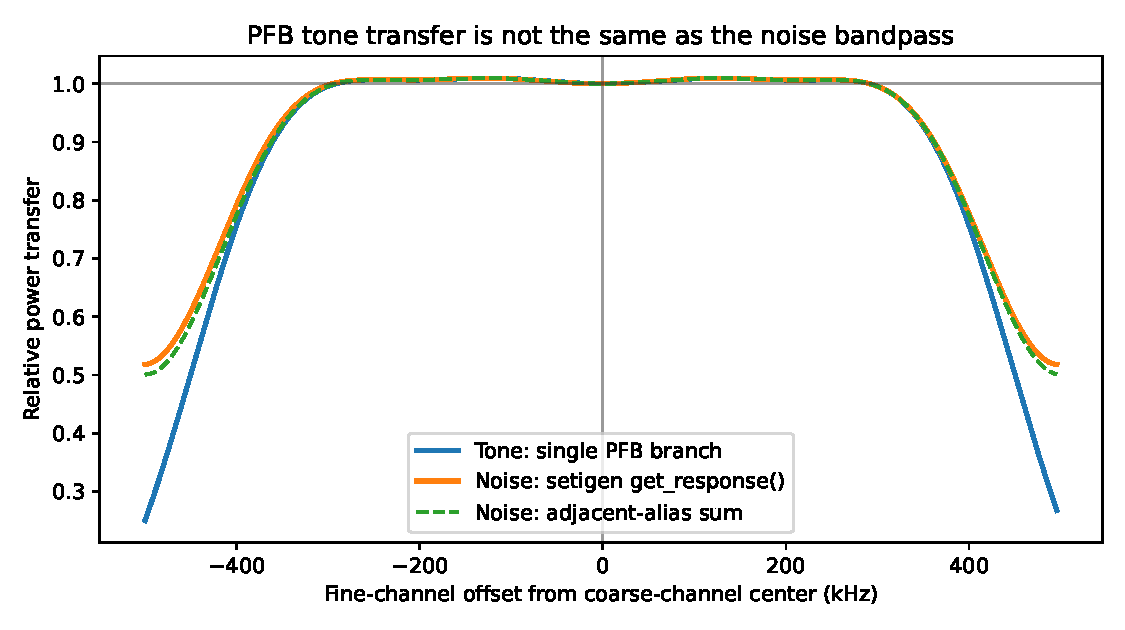
\includegraphics[width=0.9\linewidth]{figures/transfer_functions.pdf}
    \caption{The single-branch tone transfer and the aliased noise bandpass are
    different transfer functions.  At the coarse-channel edge, the noise
    bandpass remains near $0.52$ of center, while the deterministic tone branch
    response is near $0.25$ of center.}
\end{figure}

\begin{figure}[h]
    \centering
    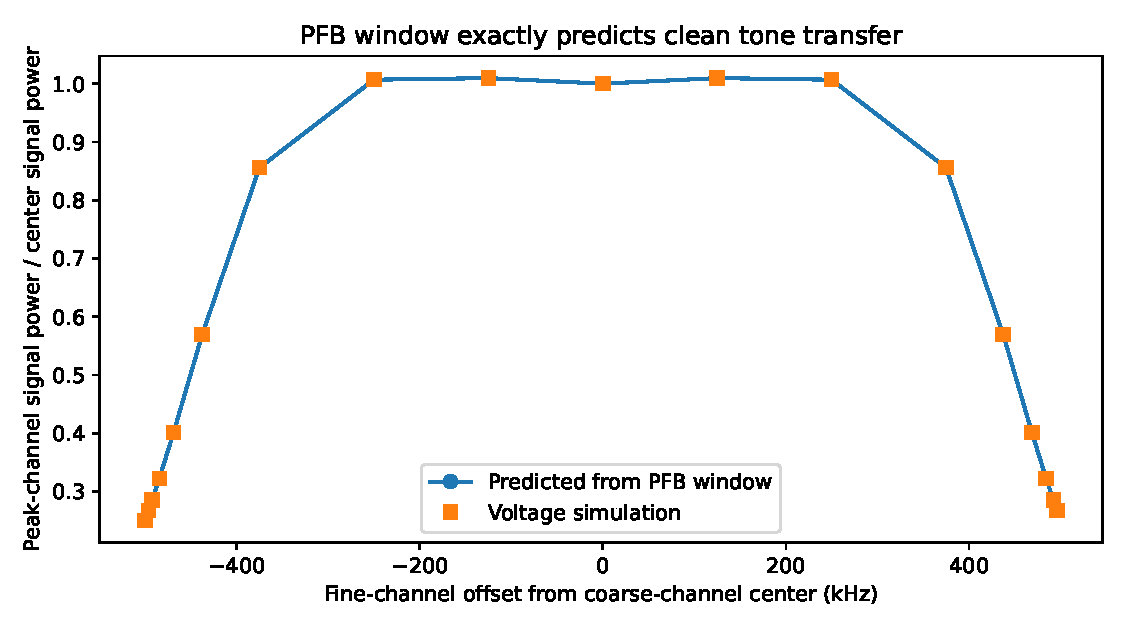
\includegraphics[width=0.9\linewidth]{figures/signal_prediction.pdf}
    \caption{The PFB-window prediction for clean tone transfer matches the
    voltage simulation.  The maximum absolute error over the tested bins is
    $1.7\times 10^{-5}$ in center-normalized power.}
\end{figure}

\begin{figure}[h]
    \centering
    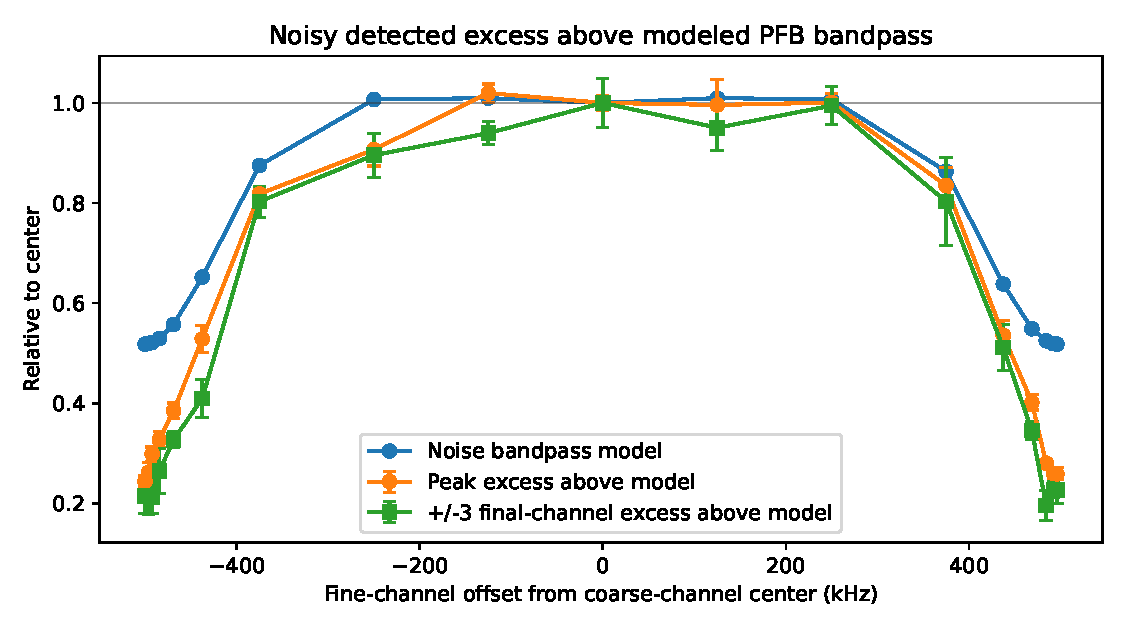
\includegraphics[width=0.9\linewidth]{figures/modeled_bandpass_excess.pdf}
    \caption{Noisy detected excess after subtracting a scaled modeled PFB
    bandpass.  The edge tone is weaker than one would infer from the noise
    bandpass alone, matching the single-branch signal-transfer prediction.}
\end{figure}

\section{Numerical Summary}

For the exact coarse-channel edge in the default experiment:
\[
\begin{array}{ll}
\text{single-branch tone prediction} & 0.2504,\\
\text{modeled noise bandpass} & 0.5179,\\
\text{noisy peak excess above modeled bandpass} & 0.2433 \pm 0.0117,\\
\text{noisy } \pm 3 \text{ final-channel aperture excess} & 0.2140 \pm 0.0336.
\end{array}
\]
All quantities are normalized to a tone at the center of the same coarse
channel.  The peak-channel detected excess agrees with the single-branch PFB
prediction, not with the noise-bandpass response.

\section{Interpretation}

The coarse-channel edge discrepancy is expected signal-processing behavior, not
a numerical accident.  The PFB is critically sampled.  Noise is stochastic and
broadband, so after decimation its fine-channelized baseline contains aliased
power from adjacent spectral images of the prototype filter.  A narrowband tone
at a known frequency is not a broadband stochastic field.  In the target
analysis branch, its detected power is controlled by the one branch response at
that frequency.  Therefore a correction curve inferred from the noise bandpass
is not sufficient to recover the original signal intensity of a narrowband tone.

Equivalently:
\[
    I_{\mathrm{noise\ baseline}}(f) \propto R_{\mathrm{noise}}(f),
    \qquad
    I_{\mathrm{tone\ excess}}(f) \propto R_{\mathrm{tone}}(f).
\]
Near the center of a coarse channel these responses are similar enough that the
difference is small.  Near a coarse-channel edge they diverge by roughly a
factor of two in power for this configuration.

\section{Implications for setigen and Real Observations}

The voltage pipeline is accurately modeling the PFB that it implements: the
same PFB window predicts the measured tone response essentially exactly.  The
remaining question is whether the implemented PFB parameters and downstream
reduction path match a given real instrument and product.  For real
observations, the calibration depends on the actual PFB coefficients, tap count,
coarse-channel selection, quantization/requantization behavior, fine FFT,
normalization, and any later bandpass flattening.

For scientific use, we should maintain two separate concepts:
\begin{enumerate}
    \item A noise-bandpass response, useful for modeling local background and
    PFB scalloping in noise statistics.
    \item A narrowband signal-transfer response, useful for recovering original
    signal intensity from detected excess.
\end{enumerate}
Using the noise-bandpass model alone would overestimate the recovered original
intensity of edge-channel narrowband signals.  The appropriate correction for a
peak-channel detector is approximately
\[
    I_{\mathrm{original}} \approx
    \frac{I_{\mathrm{detected}} - I_{\mathrm{modeled\ bandpass}}}
         {R_{\mathrm{tone}}(\delta)} ,
\]
with additional factors for off-bin fine-FFT leakage, drift smearing, and the
chosen detection aperture.

\section{Recommended Next Steps}

\begin{itemize}
    \item Expose or document both response curves in the voltage tooling:
    \texttt{noise\_response} and \texttt{tone\_response}.
    \item Repeat this experiment through the full RAW write/read/reduce path and
    with quantization enabled.
    \item Compare the implemented PFB window and response against rawspec and
    known instrument configurations.
    \item Add off-bin and drifting tones so the correction includes fine-FFT
    sinc leakage and drift-smearing effects.
    \item For real observations, estimate continuum/bandpass shape locally but
    correct narrowband signal intensity using the signal-transfer curve, not the
    noise-bandpass curve.
\end{itemize}

\end{document}
